
%-------------------------
\subsubsection*{Plane strain}

In polar coordinates the surface element is 
\[
dS = R d\theta
\]
so that 
$\int_0^{2\pi} dS = \int_0^{2\pi} R d\theta = 2 \pi R$ which is the perimeter of the circle.

We wish to normalise the pressure so that it is on average zero on the surface:
\[
p_{normalised} = p - <p>
\]
where 
\[
<p> 
= \frac{\int p(r, \theta) dS }{\int dS}
= \frac{\int p(\theta) R d\theta }{\int R d \theta d\theta}
= \frac{1}{2 \pi R} R \int p(\theta) d\theta 
= \frac{1}{2 \pi }  \int_0^{2\pi} p(\theta) d\theta 
\]
This integral is broken up in a summation over element edges which are at the surface.
\[
<p>= \frac{1}{2\pi} \sum_{e}^{nelt} \int_{\theta_{2}^e}^{\theta_{3}^e} p (\theta) d\theta
\]
where $\theta_2^e$ and $\theta_3^e$ are the $\theta$ values of nodes 2 and 3 of element $e$ that lie on the surface.
These edge integrals are simplifed by assuming a 1-point quadrature:
\[
<p>= \frac{1}{2\pi} \sum_{e}^{nelt}  p (\frac{\theta_2^e+\theta_3^e}{2}) (\theta_3^e-\theta_2^e)
\]



%------------------------------
\subsubsection*{Axisymmetric case}

\begin{center}
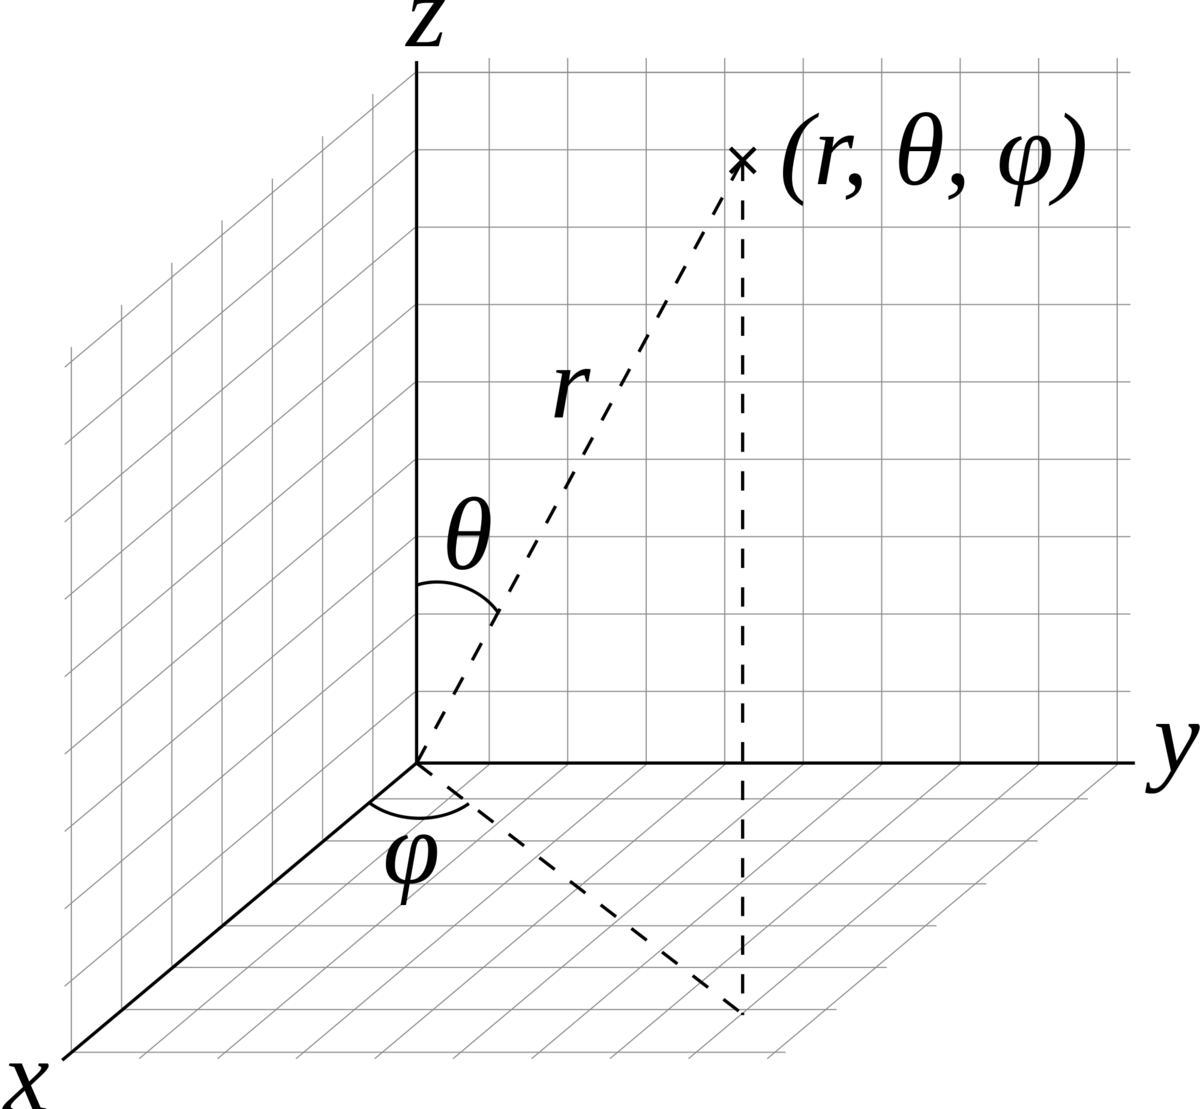
\includegraphics[width=3cm]{images/sphcoord}
\end{center}

In spherical coordinates, the surface element is 
\[
dS= R^2 \sin \theta d\theta d\phi
\]
We wish to normalise the pressure so that it is on average zero on the surface:
\[
p_{normalised} = p - <p>
\]
where 
\[
<p> 
= \frac{\iint p(\theta,\phi) dS }{\iint dS}
= \frac{\iint p(\theta,\phi) R^2 \sin \theta d\theta d\phi}{\iint R^2 \sin \theta d\theta d\phi}
\]
and since $p$ is independent of $\phi$ then 
\[
<p> 
= \frac{R_2^2 \cdot 2\pi \cdot  \int_0^\pi p(\theta)  \sin \theta d\theta}
{R_2^2 \cdot 2\pi \cdot \int  \sin \theta d\theta }
= \frac{ 2\pi R_2^2 \int_0^\pi p(\theta)  \sin \theta d\theta} {4\pi R_2^2}
\]
The integral over $\theta$ can be simplified by using the average pressure 
along the edge and the angle of the edge middle point:
\begin{lstlisting}
poffset=0
for iel in range(0,nel):
    if surface_element[iel]:
       dtheta=theta_sph[iconV[2,iel]]-theta_sph[iconV[3,iel]]
       pmean=0.5*(p[iconP[2,iel]]+p[iconP[3,iel]])
       poffset+=np.sin((theta_sph[iconV[2,iel]]+theta_sph[iconV[3,iel]])/2)*dtheta\
                *2*np.pi*R2**2 * pmean
poffset/=4*np.pi*R2**2
\end{lstlisting}

